\documentclass[../../main.tex]{subfiles}
\begin{document}

\begin{flushright}
\footnotesize\textit{【自動文字起こし・要確認】}
\end{flushright}

\noindent
\textbf{[解]} $y \ge \dfrac{1}{2} x^2, \dfrac{x^2}{1/2} + \dfrac{y^2}{1/32} \le 1$ を図示すると下図斜線部。

\begin{center}
\begin{tikzpicture}[scale=2.2, >=stealth]
  \draw[->] (-1.0, 0) -- (1.0, 0) node[right] {$x$};
  \draw[->] (0, -0.3) -- (0, 0.4) node[above] {$y$};
  \node[below left] at (0,0) {$0$};
  
  \draw[domain=-0.7:0.7, smooth, variable=\x] plot ({\x}, {0.5*\x*\x});
  \node[above right] at (0.45, 0.1) {$y = \dfrac{1}{2}x^2$};
  
  \draw[dashed] (0,0) ellipse ({1/sqrt(2)} and {1/sqrt(32)});
  
  \begin{scope}
    \clip (0,0) ellipse ({1/sqrt(2)} and {1/sqrt(32)});
    \fill[gray!30, domain=-0.7:0.7, variable=\x] (-0.7, 0.4) -- plot ({\x}, {0.5*\x*\x}) -- (0.7, 0.4) -- cycle;
  \end{scope}
  \draw[domain=-0.5:0.5, smooth, variable=\x] plot ({\x}, {0.5*\x*\x});
  \draw[dashed] (0,0) ellipse ({1/sqrt(2)} and {1/sqrt(32)});
  
  \node at (0, 0.12) {$S$};
  \node[below] at ({1/sqrt(2)}, 0) {$\dfrac{1}{\sqrt{2}}$};
  \node[below] at ({-1/sqrt(2)}, 0) {$-\dfrac{1}{\sqrt{2}}$};
  \node[below] at (0.5, 0) {$\dfrac{1}{2}$};
  \node[below] at (-0.5, 0) {$-\dfrac{1}{2}$};
  \node[above left] at (0, {1/sqrt(32)}) {$\dfrac{1}{\sqrt{32}}$};
\end{tikzpicture}
\end{center}

\noindent
(1) 対称性から
\begin{align}
\dfrac{1}{\pi} \dfrac{1}{2} V_1 &= \int_0^{\dfrac{1}{2}} \left[ \left( \dfrac{1}{32} - \dfrac{x^2}{16} \right) - \dfrac{1}{4} x^4 \right] dx \\
&= \left[ -\dfrac{1}{20} x^5 - \dfrac{1}{48} x^3 + \dfrac{1}{32} x \right]_0^{\dfrac{1}{2}} \\
&= \dfrac{11}{15} \left(\dfrac{1}{2}\right)^6
\end{align}

\[
\dfrac{1}{\pi} V_2 = \int_0^{\dfrac{1}{8}} (2y) dy + \int_{\dfrac{1}{8}}^{\dfrac{1}{\sqrt{32}}} \left( \dfrac{1}{2} - 16y^2 \right) dy
\]
\[
= \left[ y^2 \right]_0^{\dfrac{1}{8}} + \left[ \dfrac{1}{2} y - \dfrac{16}{3} y^3 \right]_{\dfrac{1}{8}}^{\dfrac{1}{\sqrt{32}}}
\]
\[
= \dfrac{1}{64} + \dfrac{1}{8} \dfrac{\sqrt{2}-1}{2} - \dfrac{16}{3} \dfrac{2\sqrt{2}-1}{8^3}
\]
\[
= \dfrac{1}{64} + \dfrac{\sqrt{2}-1}{16} - \dfrac{1}{3} \dfrac{2\sqrt{2}-1}{32}
\]
\[
= \dfrac{1}{3} \dfrac{1}{64} \left[ -7 + 8\sqrt{2} \right]
\]

だから
\[
V_1 = \dfrac{11}{15} \left(\dfrac{1}{2}\right)^5 \pi, \quad V_2 = \dfrac{\pi}{192} (-7 + 8\sqrt{2})
\]

\bigskip

\noindent
(2) (1) から、
\begin{align}
\dfrac{V_2}{V_1} &= \dfrac{\dfrac{1}{3} \left(\dfrac{1}{2}\right)^6 (-7 + 8\sqrt{2})}{\dfrac{11}{15} \left(\dfrac{1}{2}\right)^5} = \dfrac{\dfrac{1}{6}(-7 + 8\sqrt{2})}{\dfrac{11}{15}} \\
&= \dfrac{5}{22} (-7 + 8\sqrt{2}) < 1 \\
&\iff -7 + 8\sqrt{2} < \dfrac{22}{5} \iff 8\sqrt{2} < \dfrac{57}{5} \quad \cdots \textcircled{1}
\end{align}
だが、①は $64 \cdot 2 \cdot 25 = 3200 < 3249 = (57)^2$ の平方根をとって
$8\sqrt{2} < \dfrac{57}{5}$ だから成立。よって
\[ \dfrac{V_2}{V_1} < 1 \]

\bigskip

\end{document}
